\documentclass[11pt]{article}

\usepackage[letterpaper,bindingoffset=0.2in,
            left=1in,right=1in,top=1in,bottom=1in,
            footskip=.25in]{geometry}

\usepackage{hyperref}
	\hypersetup{
			colorlinks=true,
			linkcolor=black,
			filecolor=magenta,      
			urlcolor=blue,
	}
	
\usepackage{graphicx}
	\graphicspath{ {images/} }
	
\begin{document}

\title{COMP SCI 5401 FS2017 Assignment 1b}
\author{Stuart Miller\\\href{mailto:sm67c@mst.edu}{sm67c@mst.edu}}
\maketitle

\section{Fitness Plots}

\begin{center}
Instance 1\\
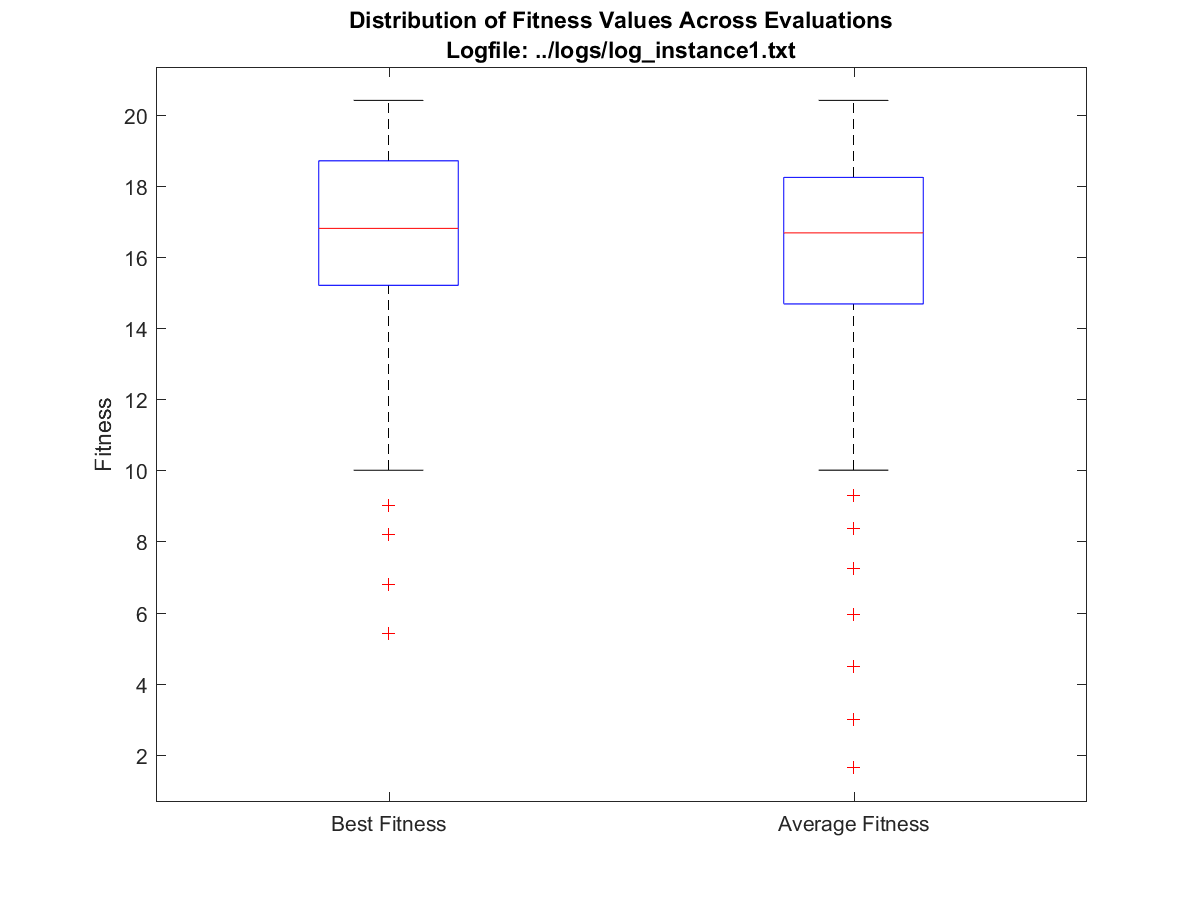
\includegraphics[width=5in]{graph_1.png}\\
\newpage Instance 2\\
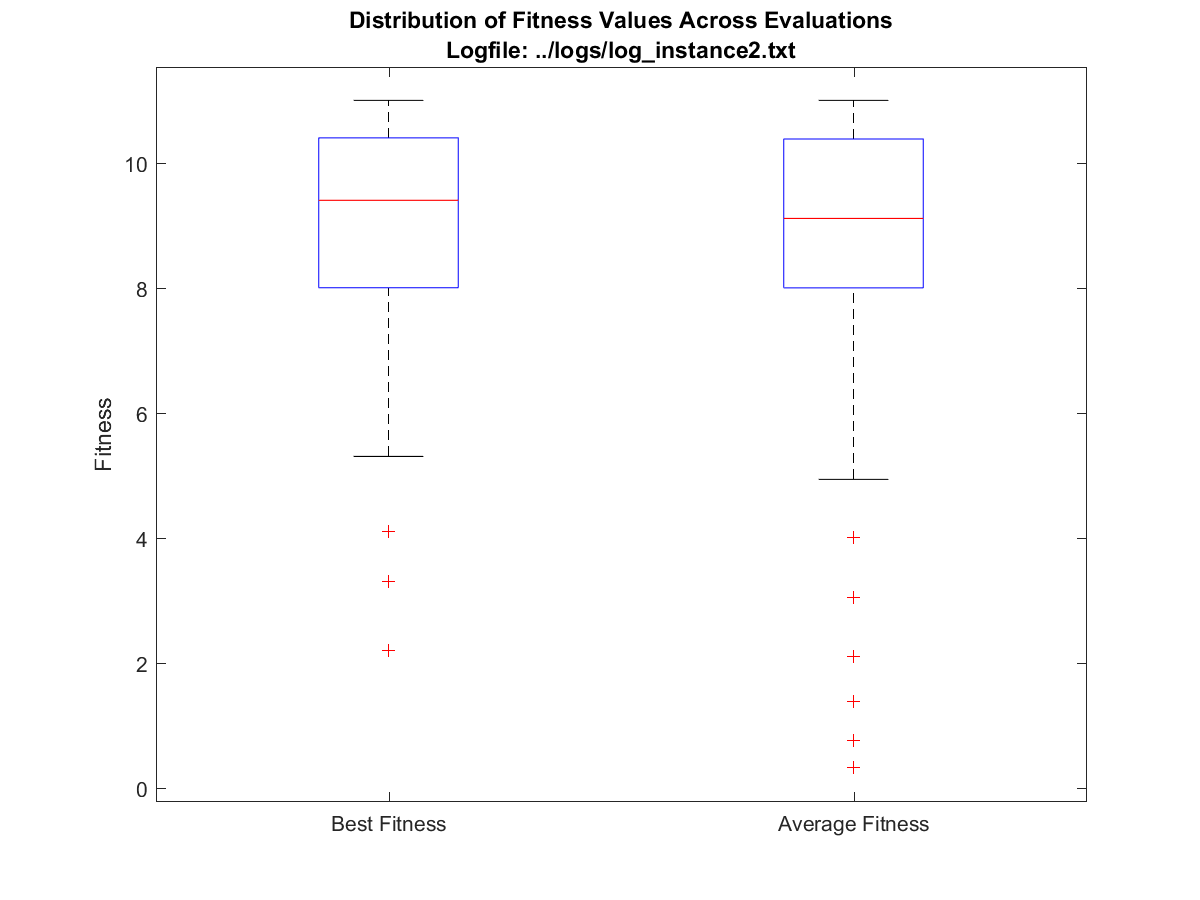
\includegraphics[width=5in]{graph_2.png}\\
Instance 3\\
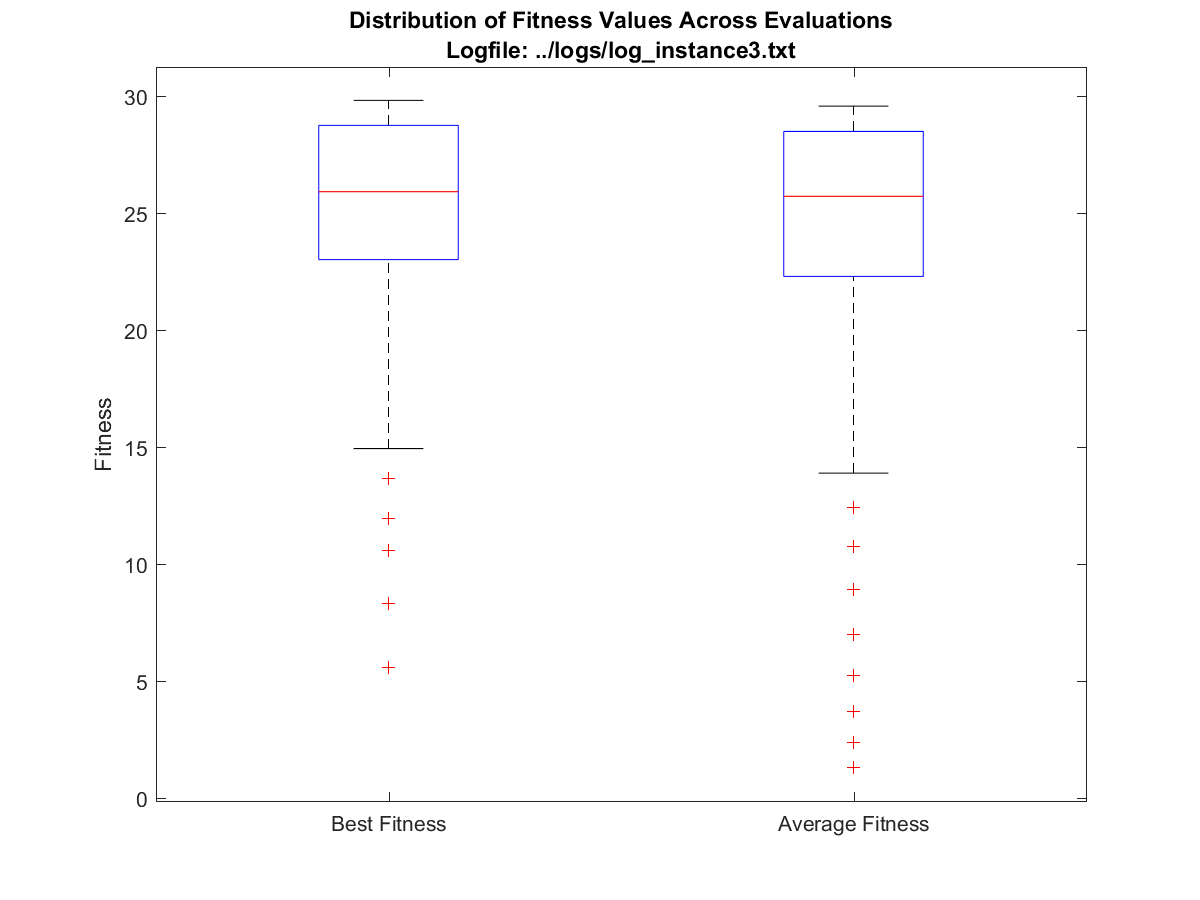
\includegraphics[width=5in]{graph_3.png}\\
\end{center}

\newpage \section{Statistical Analysis}
\begin{center}
Instance 1\\
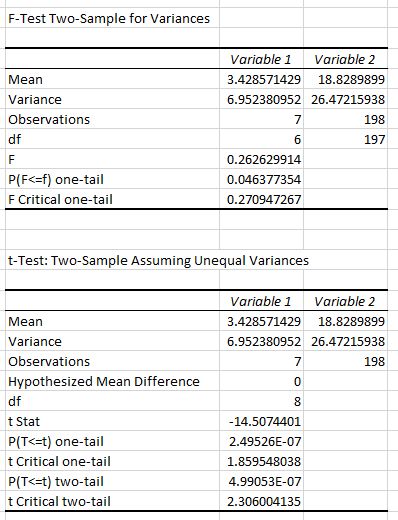
\includegraphics[width=3in]{stat_anal_1.png}\\
Instance 2\\
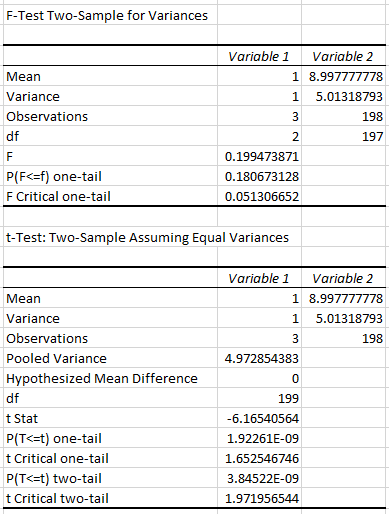
\includegraphics[width=3in]{stat_anal_2.png}\\
\newpage Instance 3\\
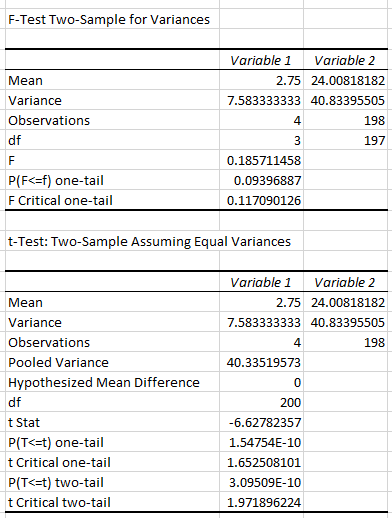
\includegraphics[width=3in]{stat_anal_3.png}\\
\end{center}

\section{Bonus 1 - Operator Comparison}\indent

For the operator comparison, both n-point and uniform crossover methods were implemented for the recombination stage and random reset and creep methods were implemented for the mutation stage. The parameters were set to 3 crossover points (for n-point crossover), 50\% distribution (for uniform crossover), creep distance of 2 (for creep mutation), and a 20\% mutation chance. The limit of 10,000 fitness evaluations was kept, but increased to 100 runs for more data. The best solution from each run was kept and plotted as show below. Trendlines and labels were added to show averages for each.

As shown in the plots below, uniform crossover tends to perform slightly better, while random reset mutation consistently outperforms creep mutation.
\begin{center}
	\newpage Recombination\\
	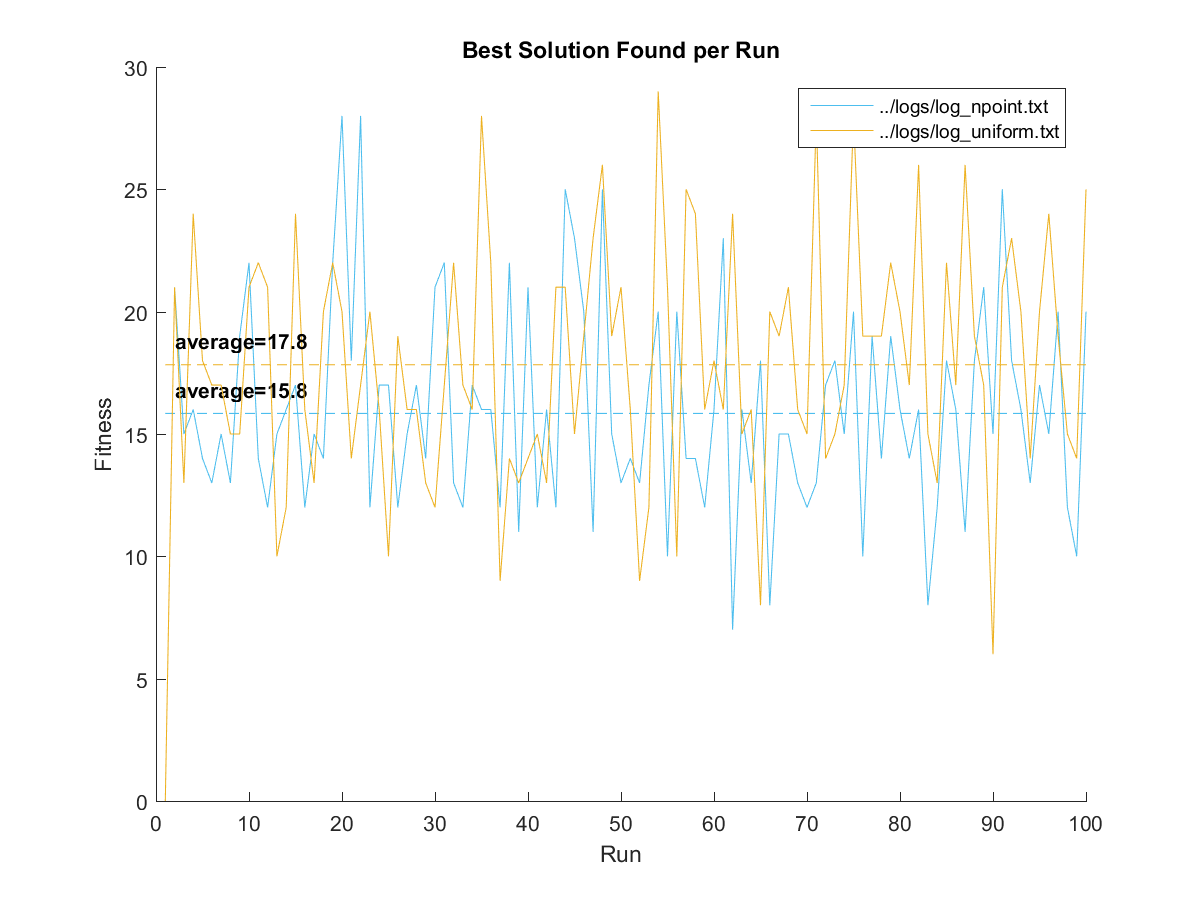
\includegraphics[width=5in]{graph_bonus1_recombination.png}
\end{center}
\begin{center}
	Mutation\\
	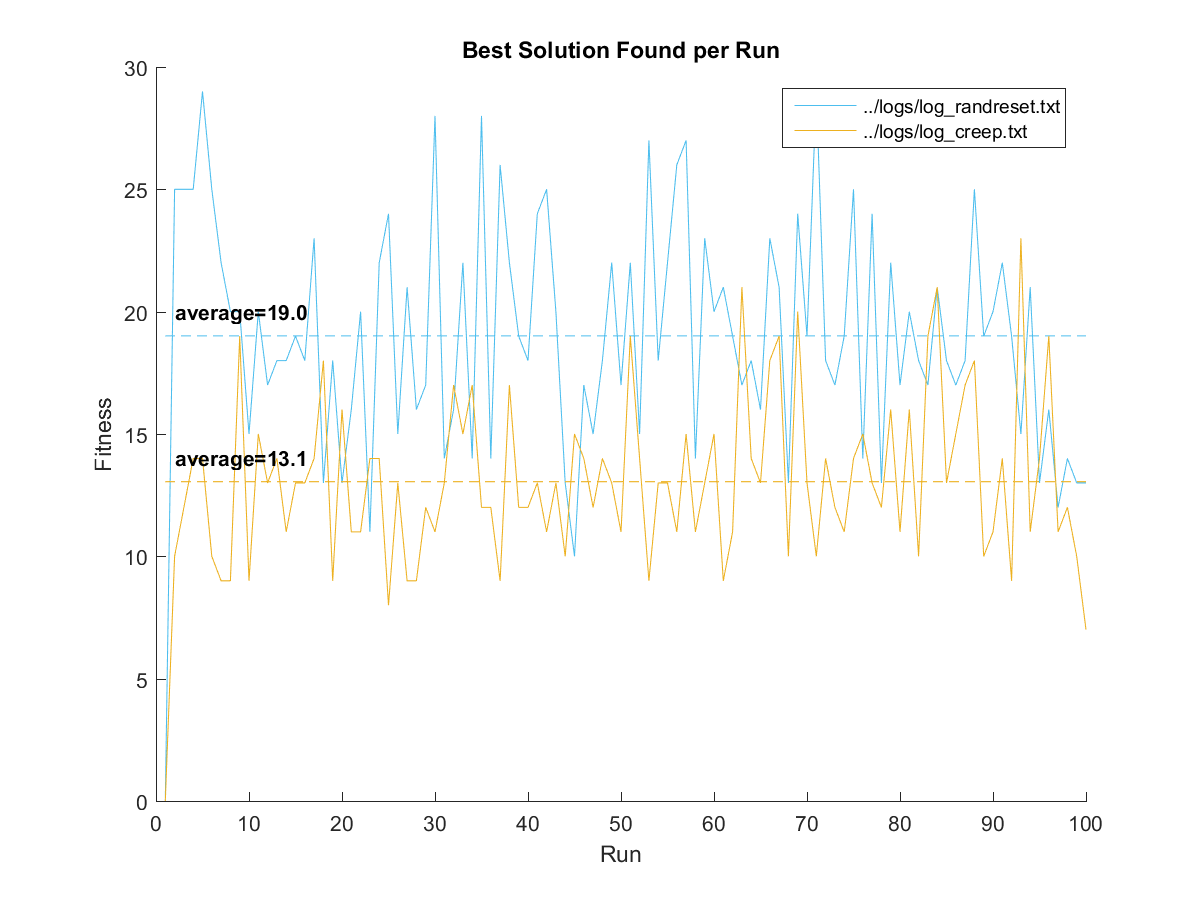
\includegraphics[width=5in]{graph_bonus1_mutation.png}
\end{center}
	
\newpage\section{Bonus 2 - Repair Function}\indent
	
For repair function analysis, the same configuration was used as Bonus 1. Recombination was set to uniform and mutation was set to random reset and these were determined to be best performing. In initial testing, the repair function always outperformed random placements, so a configuration option was not added to turn it off. For the control in this experiment, the code was manually altered to assign random placements until valid instead of attempting a repair. 

As you can see, the non-repairing version performs much worse.

\begin{center}
	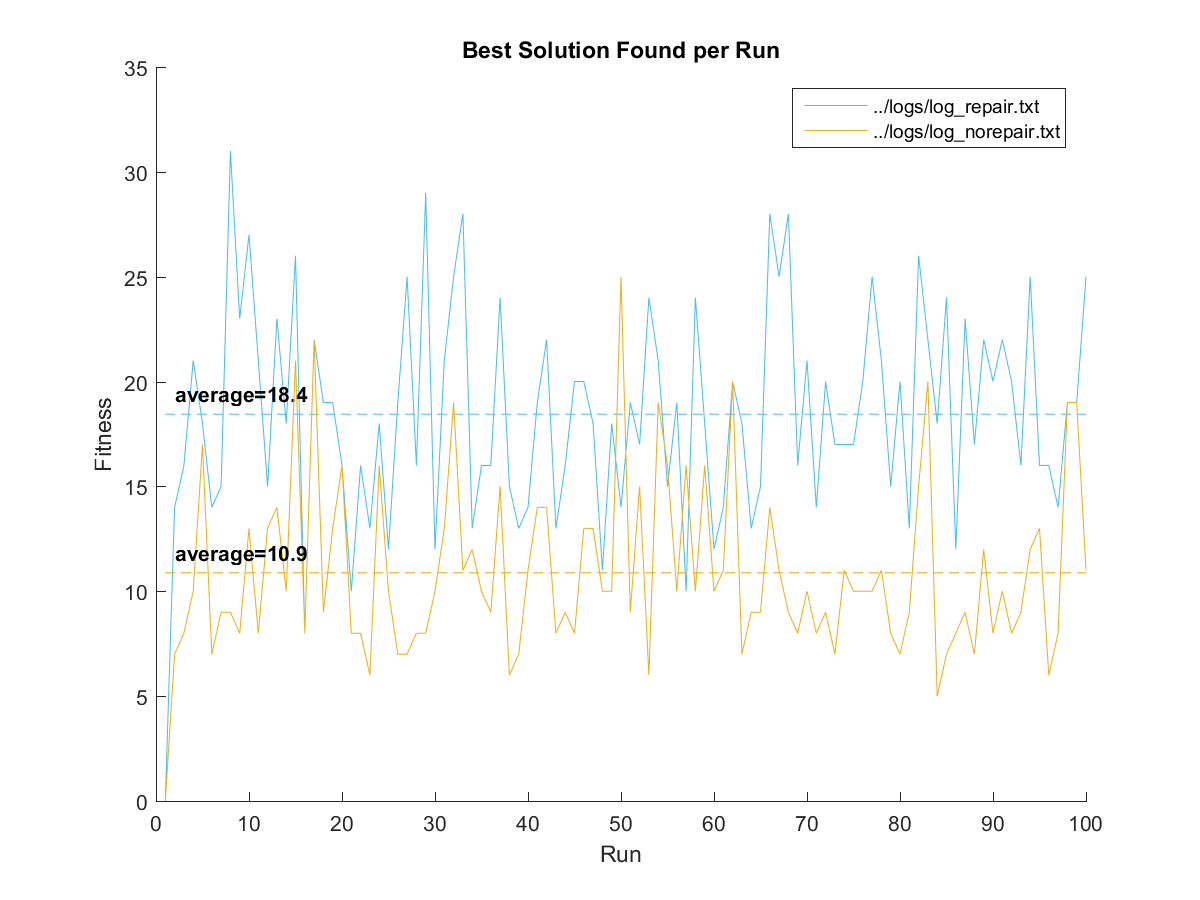
\includegraphics[width=5in]{graph_bonus2_repair.png}
\end{center}

\end{document}